\documentclass{beamer}
\usepackage{graphicx}
\usepackage{xcolor}
\usepackage{tikz}
\usepackage{amsmath}

% 自定义颜色
\definecolor{purpleblue}{RGB}{80, 80, 180}
\definecolor{lightgray}{RGB}{230, 230, 230}
\definecolor{novelPurple}{RGB}{98, 54, 255} 
\definecolor{darkgray}{RGB}{50, 50, 50}

% 主题设置
\usetheme{Madrid}  
\usecolortheme{dolphin} 

% 设置字体
\setbeamerfont{title}{size=\Large,series=\bfseries}
\setbeamerfont{frametitle}{size=\LARGE,series=\bfseries}
\setbeamercolor{frametitle}{fg=white, bg=novelPurple}
\setbeamercolor{title}{fg=white, bg=purpleblue}

% 封面信息
\title[SAT Unit 1.2 Linear Function]{\textbf{SAT Unit 1.2 \\ Linear Function}}
\author{\textbf{Jack Zeng}}
\institute{\textcolor{white}{\textbf{Novel Prep}}}
\date{\today} 

\begin{document}

% --- Title Slide ---
\begin{frame}
    \titlepage
    \vfill
    \begin{flushright}
        \textcolor{purpleblue}{\Huge \textbf{Novel Prep}}
    \end{flushright}
\end{frame}

% --- Custom Background Slide ---
\begin{frame}
    \begin{tikzpicture}[remember picture, overlay]
        % 设置浅色渐变背景
        \shade[top color=softPurple, bottom color=softGray] 
            (current page.north west) rectangle (current page.south east);
        
        % 添加高斯模糊光晕
        \fill[white, opacity=0.3] (current page.center) circle (4cm);
        
        % 主标题
        \node[align=center] at (current page.center) {
            {\Huge\bfseries\textcolor{purpleblue}{Novel Prep}} \\[0.5cm]
            {\Large\itshape\textcolor{lightText}{Excellence in SAT Prep}}
        };

        % 添加柔和光点（点缀）
        \foreach \x in {1,2,3,4,5} {
            \fill[purpleblue, opacity=0.2] (rand*10-5, rand*7-3.5) circle (0.1+\x*0.05);
        }

        ;
    \end{tikzpicture}
\end{frame}

\begin{frame}{Overview}
    \tableofcontents
\end{frame}


\begin{frame}
\section{Linear Function}
    \begin{tikzpicture}[remember picture, overlay]
        \shade[top color=softPurple, bottom color=softGray] 
            (current page.north west) rectangle (current page.south east);
        \fill[white, opacity=0.3] (current page.center) circle (4cm);
        \node[align=center] at (current page.center) {
            {\huge\bfseries\textcolor{purpleblue}{Linear Function}} \\[0.5cm]
            {\large\itshape\textcolor{lightText}{Excellence in SAT Prep}}
        };
        \foreach \x in {1,2,3,4,5} {
            \fill[purpleblue, opacity=0.2] (rand*10-5, rand*7-3.5) circle (0.1+\x*0.05);
        }
        ;
    \end{tikzpicture}
\end{frame}
% --- Introduction to Linear Functions ---
\begin{frame}{Linear Functions}
    \begin{itemize}
        \item A linear function is an equation that models a \textbf{straight line}.
        \item General form: 
        \[
        f(x) = mx + b
        \]
        where \( m \) is the slope and \( b \) is the y-intercept.
        \item Properties:
        \begin{itemize}
            \item Constant rate of change.
            \item Graph is a straight line.
            \item Slope \( m \) determines the steepness.
        \end{itemize}
    \end{itemize}
\end{frame}


\begin{frame}{Evaluating Functions}
    \textbf{Topic: Evaluating a Function at a Given Input}

    \begin{itemize}
        \item A function such as \( h(x) = 4x - 9 \) describes a relationship between input \(x\) and output \(h(x)\).
        \item To evaluate the function at a specific value (e.g., \(x = -3\)), substitute that value into the expression.
        \item Carefully apply arithmetic operations: multiplication first, then addition/subtraction.
        \item This process gives the function's output for that input, also known as the value of the function.
    \end{itemize}

    \vspace{1em}
    \textbf{Key Skill:}  
    Mastery of function evaluation builds the foundation for function tables, graphing, and understanding function behavior.
\end{frame}









% --- Question 2 ---
\begin{frame}{Question : X-Intercept of Combined Functions}
    The functions \( f \) and \( g \) are defined as:
    \[
    f(x) = \frac{1}{4}x - 9, \quad g(x) = \frac{3}{4}x + 21.
    \]
    If the function \( h \) is defined as:
    \[
    h(x) = f(x) + g(x),
    \]
    what is the x-coordinate of the x-intercept of the graph of \( y = h(x) \) in the \( xy \)-plane?
\end{frame}
% --- Slide: Definition of Slope and Real-World Examples ---

\begin{frame}
    \begin{tikzpicture}[remember picture, overlay]
        \shade[top color=softPurple, bottom color=softGray] 
            (current page.north west) rectangle (current page.south east);
        \fill[white, opacity=0.3] (current page.center) circle (4cm);
        \node[align=center] at (current page.center) {
            {\huge\bfseries\textcolor{purpleblue}{Slope}} \\[0.5cm]
            {\large\itshape\textcolor{lightText}{Excellence in SAT Prep}}
        };
        \foreach \x in {1,2,3,4,5} {
            \fill[purpleblue, opacity=0.2] (rand*10-5, rand*7-3.5) circle (0.1+\x*0.05);
        }
        ;
    \end{tikzpicture}
\end{frame}
\begin{frame}{Understanding Slope}
\section{Slope}

    \textbf{Definition:}  
    The \textbf{slope} of a line measures the steepness and direction of the line. It is represented as:

    \[
    m = \frac{\Delta y}{\Delta x} = \frac{y_2 - y_1}{x_2 - x_1}
    \]

    where:
    \begin{itemize}
        \item \( m \) is the slope,
        \item \( (x_1, y_1) \) and \( (x_2, y_2) \) are two points on the line,
        \item \( \Delta y \) represents the vertical change (rise),
        \item \( \Delta x \) represents the horizontal change (run).
    \end{itemize}

    \vspace{0.5cm}
    \textbf{Real-World Applications of Slope:}
    \begin{itemize}
        \item \textbf{Road Inclines:} The slope of a highway ramp or a hill indicates how steep the road is.
        \item \textbf{Construction:} Roofs have slopes to allow rainwater to flow off properly.

    \end{itemize}

\end{frame}


\begin{frame}{Understanding Slope Visually}
    \textbf{Slope (\(m\)) measures the steepness and direction of a line.}

    \begin{columns}
        \column{0.5\textwidth}
        \begin{itemize}
            \item Formula: \( m = \frac{y_2 - y_1}{x_2 - x_1} \)
            \item Also called: \textbf{rise over run}
            \item Positive slope: line rises from left to right
            \item Negative slope: line falls from left to right
        \end{itemize}

        \column{0.5\textwidth}
        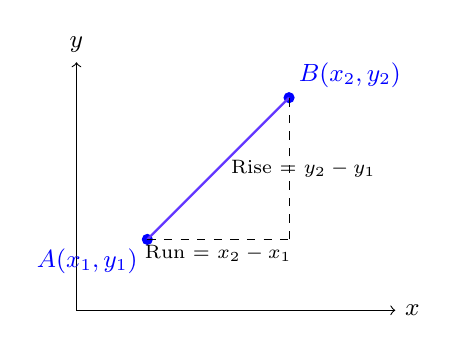
\begin{tikzpicture}[scale=0.9]
            \draw[->] (0,0) -- (4.5,0) node[right] {\small \(x\)};
            \draw[->] (0,0) -- (0,3.5) node[above] {\small \(y\)};

            % Points
            \filldraw[blue] (1,1) circle (2pt) node[below left] {\small \(A(x_1, y_1)\)};
            \filldraw[blue] (3,3) circle (2pt) node[above right] {\small \(B(x_2, y_2)\)};

            % Line
            \draw[thick, novelPurple] (1,1) -- (3,3);

            % Rise and Run
            \draw[dashed] (1,1) -- (3,1);
            \draw[dashed] (3,1) -- (3,3);

            \node at (2,0.8) {\scriptsize Run = \(x_2 - x_1\)};
            \node at (3.2,2) {\scriptsize Rise = \(y_2 - y_1\)};
        \end{tikzpicture}
    \end{columns}

    \vspace{1em}
    \centering
    \textcolor{gray}{Slope shows how much \(y\) increases or decreases as \(x\) increases.}
\end{frame}


% --- Question 3 ---
\begin{frame}{Question : Temperature Conversion}
    The function \( F \) gives the temperature, in degrees Fahrenheit, that corresponds to a temperature of \( x \) kelvins:
    \[
    F(x) = \frac{9}{5} (x - 273.15) + 32.
    \]
    If a temperature increased by \textbf{2.1} kelvins, by how much did the temperature increase, in degrees Fahrenheit?
    \[
    \begin{array}{ll}
    \textbf{A.} & 3.78 \\
    \textbf{B.} & 35.78 \\
    \textbf{C.} & 487.89 \\
    \textbf{D.} & 519.89
    \end{array}
    \]
\end{frame}

\begin{frame}{\textbf{Question: Meaning of the Constant in the Equation}}
    An object hangs from a spring. The formula
    \[
    \ell = 30 + 2w
    \]
    relates the length \( \ell \), in centimeters, of the spring to the weight \( w \), in newtons, of the object.

    Which of the following describes the meaning of the \( 2 \) in this context?

    \vspace{0.5cm}
    \textbf{Options:}
    \begin{enumerate}
        \item[A.] The length, in centimeters, of the spring with no weight attached.
        \item[B.] The weight, in newtons, of an object that will stretch the spring 30 centimeters.
        \item[C.] The increase in the weight, in newtons, of the object for each one-centimeter increase in the length of the spring.
        \item[D.] The increase in the length, in centimeters, of the spring for each one-newton increase in the weight of the object.
    \end{enumerate}
\end{frame}

% --- Answer Explanation ---
\begin{frame}{\textbf{Answer Explanation: Meaning of the Constant in the Equation}}
    \textbf{Correct Answer: \textcolor{novelPurple}{\( \mathbf{D} \)}}  

    \vspace{0.3cm}
    \textbf{Solution:}
    \begin{itemize}
        \item The given equation is \( \ell = 30 + 2w \).
        \item The coefficient \( 2 \) represents the rate at which the length of the spring increases as the weight increases.
        \item This means that for each additional newton of weight, the length of the spring increases by \( 2 \) centimeters.
    \end{itemize}

    \textbf{Final Answer:} \( \boxed{\text{D}} \).
\end{frame}


\begin{frame}

\section{Graphs of Linear Function}
    \begin{tikzpicture}[remember picture, overlay]
        \shade[top color=softPurple, bottom color=softGray] 
            (current page.north west) rectangle (current page.south east);
        \fill[white, opacity=0.3] (current page.center) circle (4cm);
        \node[align=center] at (current page.center) {
            {\LARGE\bfseries\textcolor{purpleblue}{Graphs and Applications of Linear Function}} \\[0.5cm]
            {\large\itshape\textcolor{lightText}{Excellence in SAT Prep}}
        };
        \foreach \x in {1,2,3,4,5} {
            \fill[purpleblue, opacity=0.2] (rand*10-5, rand*7-3.5) circle (0.1+\x*0.05);
        }
        ;
    \end{tikzpicture}
\end{frame}


\begin{frame}{Graphing a Linear Function}
    \textbf{Example:} Graph of \( f(x) = 2x - 1 \)

    \vspace{1em}
    \begin{center}
        
    
    \begin{tikzpicture}[scale=0.55]
        % Axes
        \draw[->] (-2.5, 0) -- (4.5, 0) node[right] {\small \(x\)};
        \draw[->] (0, -3.5) -- (0, 5) node[above] {\small \(y\)};

        % Grid (optional)
        \draw[step=1, gray!20, thin] (-2.4,-3.4) grid (4.4,4.9);

        % Plot line: f(x) = 2x - 1
        \draw[thick, novelPurple] (-1.5,-4) -- (3,5);

        % Key points
        \filldraw[blue] (0,-1) circle (2pt) node[below left] {\footnotesize y-intercept \((0, -1)\)};
        \filldraw[blue] (1,1) circle (2pt) node[below right] ;
        \filldraw[blue] (2,3) circle (2pt) node[below right] ;

        % Rise/run triangle from (1,1) to (2,3)
        \draw[dashed] (1,1) -- (2,1);
        \draw[dashed] (2,1) -- (2,3);

        \node at (2,0.7) {\scriptsize Run = 1};
        \node at (3.1,2) {\scriptsize Rise = 2};

        \node at (2.5,4.2) {\color{novelPurple}\scriptsize Slope \(m = \frac{2}{1} = 2\)};
    \end{tikzpicture}

    \vspace{0.5em}
    \centering
    \textcolor{gray}{A linear function graphs as a straight line. Slope and intercept define its position.}
    \end{center}
\end{frame}



\begin{frame}{Interpreting Piecewise Linear Graphs}
    \textbf{Topic: Interpreting Piecewise Linear Graphs \& Calculating Rate of Change}

    \begin{itemize}
        \item A graph showing a quantity over time helps visualize how that quantity changes.
        \item The \textbf{rate of change} (e.g., rainfall per hour) is calculated as:
        \[
        \text{Rate} = \frac{\text{Change in } y}{\text{Change in } x} = \frac{\Delta y}{\Delta x}
        \]
        \item A \textbf{horizontal segment} means the quantity is not changing during that time (rate = 0).
        \item A \textbf{steeper line} means a faster rate of change.
        \item When analyzing the graph:
        \begin{itemize}
            \item Look for intervals with different slopes.
            \item Compare slope values to find where the rate is greatest or increasing/decreasing.
        \end{itemize}
    \end{itemize}

    \vspace{1em}
    \textbf{Key Skill:}  
    Understanding graphs requires both visual reading and numerical slope calculation.
\end{frame}



\begin{frame}{Interpreting  Piecewise Linear Graphs}
    \textbf{Concept:} Use graphs to visualize how quantities change over time.

    \begin{columns}
        \column{0.5\textwidth}
        \begin{itemize}
            \item A line segment shows a constant rate of change.
            \item A steeper slope means a faster rate.
            \item A flat segment means the value is not changing (rate = 0).
            \item Rate = \( \frac{\Delta y}{\Delta x} \)
        \end{itemize}

        \column{0.5\textwidth}
        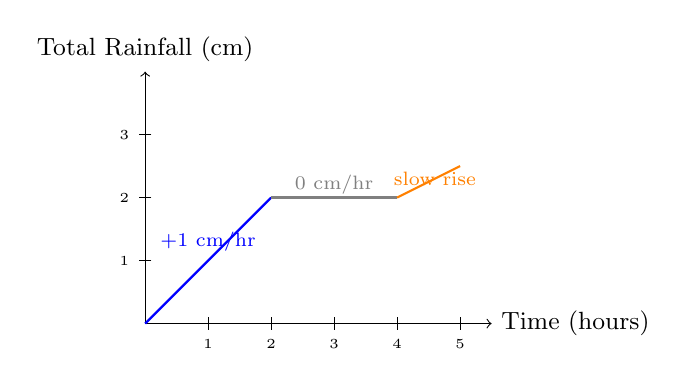
\begin{tikzpicture}[scale=0.8]
            \draw[->] (0,0) -- (5.5,0) node[right] {\small Time (hours)};
            \draw[->] (0,0) -- (0,4) node[above] {\small Total Rainfall (cm)};

            % segments
            \draw[blue, thick] (0,0) -- (2,2);
            \draw[gray, thick] (2,2) -- (4,2);
            \draw[orange, thick] (4,2) -- (5,2.5);

            % grid dots
            \foreach \x in {1,2,3,4,5}
                \draw (\x,0.1) -- (\x,-0.1) node[below] {\tiny \x};
            \foreach \y in {1,2,3}
                \draw (0.1,\y) -- (-0.1,\y) node[left] {\tiny \y};

            % rate labels
            \node[blue] at (1,1.3) {\scriptsize +1 cm/hr};
            \node[gray] at (3,2.2) {\scriptsize 0 cm/hr};
            \node[orange] at (4.6,2.3) {\scriptsize slow rise};
        \end{tikzpicture}
    \end{columns}
\end{frame}


\begin{frame}{Question : Rainfall Rate Interpretation}
\small
\begin{center}
    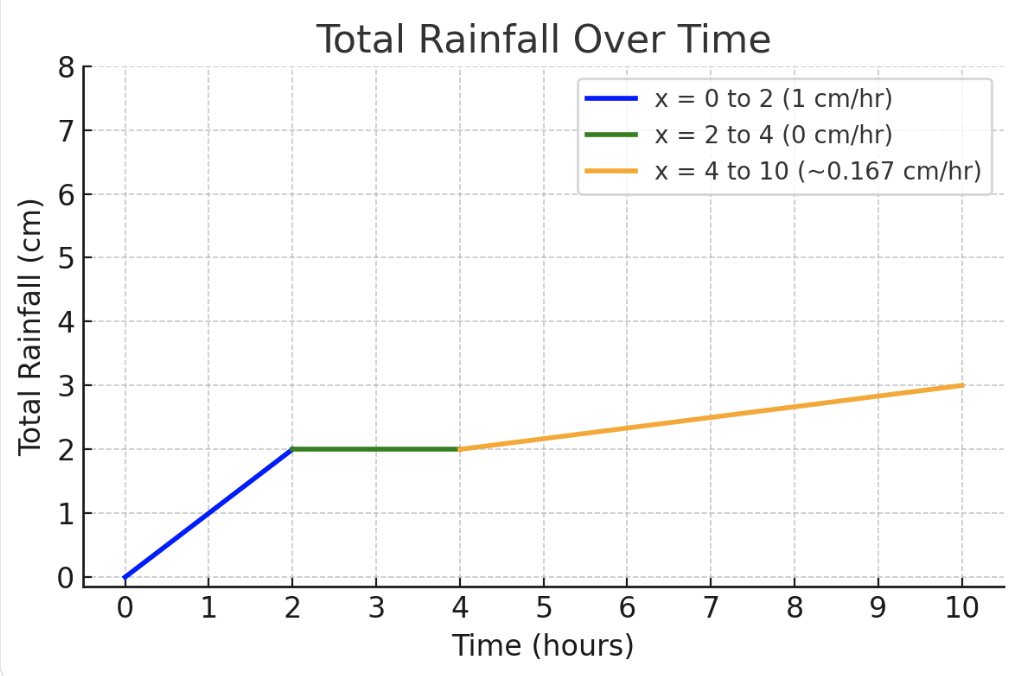
\includegraphics[width=0.4\linewidth]{E73.png}
\end{center}

    The graph shows the total amount of rainfall \(y\), in centimeters, from the start of a 10-hour period,  
    where \(x\) is the number of hours after the start of the period.

    Which of the following statements about the rainfall during this time period is true?


    \begin{itemize}
        \item[\textbf{A.}] The rate of rainfall was 2 centimeters per hour between \(x = 2\) and \(x = 4\).
        \item[\textbf{B.}] The rate of rainfall was the greatest between \(x = 4\) and \(x = 10\).
        \item[\textbf{C.}] The rate of rainfall increased between \(x = 0\) and \(x = 2\).
        \item[\textbf{D.}] The rate of rainfall was 0 centimeters per hour between \(x = 2\) and \(x = 4\).
    \end{itemize}
\end{frame}


\begin{frame}{Answer : Rainfall Rate Interpretation}
\small
    \textbf{Analyzing the Graph:}
    \begin{itemize}
        \item From \(x = 0\) to \(x = 2\):  
        \[
        \text{Rate} = \frac{2 - 0}{2 - 0} = 1 \text{ cm/hr}
        \]
        \item From \(x = 2\) to \(x = 4\):  
        \[
        \text{Rate} = \frac{2 - 2}{4 - 2} = 0 \text{ cm/hr (flat segment)}
        \]
        \item From \(x = 4\) to \(x = 10\):  
        \[
        \text{Rate} = \frac{3 - 2}{10 - 4} = \frac{1}{6} \approx 0.167 \text{ cm/hr}
        \]
    \end{itemize}

    \vspace{0.5em}
    \textbf{Evaluating the Choices:}
    \begin{itemize}
        \item \textbf{A.} Incorrect — rate was 0, not 2
        \item \textbf{B.} Incorrect — greatest rate was from \(x = 0\) to \(2\)
        \item \textbf{C.} Incorrect — rate did not increase; it was constant at 1
        \item \textbf{D.} \textbf{Correct} — rate was 0 cm/hr between \(x = 2\) and \(x = 4\)
    \end{itemize}

    \vspace{0.5em}
    \textbf{Correct Answer: D}
\end{frame}

% --- Question 1 ---
\begin{frame}{Question : Window Repair Cost}
    A window repair specialist charges \textbf{\$220} for the first two hours of repair plus an hourly fee for each additional hour. The total cost for 5 hours of repair is \textbf{\$400}. Which function \( f \) gives the total cost, in dollars, for \( x \) hours of repair, where \( x \geq 2 \)?
    \[
    \begin{array}{ll}
    \textbf{A.} & f(x) = 60x + 100 \\
    \textbf{B.} & f(x) = 60x + 220 \\
    \textbf{C.} & f(x) = 80x \\
    \textbf{D.} & f(x) = 80x + 220
    \end{array}
    \]
\end{frame}


\begin{frame}{Answer to Question }
    To determine the hourly fee, subtract the base cost from the total cost for 5 hours:
    \[
    400 - 220 = 180 \quad \Rightarrow \quad \text{for 3 extra hours}
    \]
    \[
    \text{Hourly fee} = \frac{180}{3} = 60
    \]
    So, the cost function is:
    \[
    f(x) = 220 + 60(x - 2)
    \]
    Simplifying:
    \[
    f(x) = 60x + 100
    \]
    \textbf{Correct Answer: A.} \( f(x) = 60x + 100 \)
\end{frame}


\begin{frame}
\section{Practice}
    \begin{tikzpicture}[remember picture, overlay]
        \shade[top color=softPurple, bottom color=softGray] 
            (current page.north west) rectangle (current page.south east);
        \fill[white, opacity=0.3] (current page.center) circle (4cm);
        \node[align=center] at (current page.center) {
            {\huge\bfseries\textcolor{purpleblue}{Practice}} \\[0.5cm]
            {\large\itshape\textcolor{lightText}{Excellence in SAT Prep}}
        };
        \foreach \x in {1,2,3,4,5} {
            \fill[purpleblue, opacity=0.2] (rand*10-5, rand*7-3.5) circle (0.1+\x*0.05);
        }
        ;
    \end{tikzpicture}
\end{frame}


\begin{frame}{Question: Interpreting Constants in a Function}
The given function \( h(t) = 100 - 4t \) models the number of hours until a gallon of milk held at a temperature of \( t \), in degrees Celsius, goes sour.

\vspace{0.5em}
Which of the following is the best interpretation of the number \( 4 \) in this context?

\vspace{0.5em}
\begin{itemize}
    \item[\textbf{A.}] An increase of \(1^\circ\text{C}\) will make a gallon of milk go sour 4 hours faster.
    \item[\textbf{B.}] An increase of \(1^\circ\text{C}\) will make 4 gallons of milk go sour 1 hour faster.
    \item[\textbf{C.}] An increase of \(4^\circ\text{C}\) will make a gallon of milk go sour 1 hour faster.
    \item[\textbf{D.}] An increase of \(4^\circ\text{C}\) will make a gallon of milk go sour 4 hours faster.
\end{itemize}
\end{frame}


\begin{frame}{Answer: Interpreting Constants in a Function}
\textbf{Correct Answer: \textcolor{novelPurple}{A}}  

\vspace{0.5em}
\textbf{Reasoning:}
\begin{itemize}
    \item The function is \( h(t) = 100 - 4t \), which means the number of hours until souring \emph{decreases} as temperature increases.
    \item The coefficient \( -4 \) represents the rate of change: for each \(1^\circ\text{C}\) increase in temperature, the milk sours 4 hours \textbf{sooner}.
    \item This matches exactly with Choice A.
\end{itemize}

\vspace{0.5em}
\textbf{Interpretation:}  
The number 4 means that \textbf{for every \(1^\circ\text{C}\) rise in temperature, the souring time decreases by 4 hours}.
\end{frame}


\begin{frame}{Question : Phone Plan Cost Increase}
The function \( C(x) = 0.07(x - 180) + 62.6 \) gives the monthly cost, in dollars, of using an international phone plan for \( x \) minutes each month.

\vspace{0.5em}
If the phone plan is used for 75 more minutes each month, by how many dollars does the monthly cost of the plan increase?

\begin{itemize}
    \item[\textbf{A.}] 1.75
    \item[\textbf{B.}] 5.25
    \item[\textbf{C.}] 55.25
    \item[\textbf{D.}] 67.85
\end{itemize}
\end{frame}

\begin{frame}{Answer }
\textbf{Correct Answer: \textcolor{novelPurple}{B.}}

\vspace{0.5em}
\textbf{Reasoning:}
\begin{itemize}
    \item The slope of the function is \( 0.07 \), which is the cost per additional minute.
    \item An increase of 75 minutes leads to:
    \[
    \Delta C = 0.07 \times 75 = 5.25
    \]
    \item So the cost increases by \textdollar5.25.
\end{itemize}
\end{frame}

\begin{frame}{Question : Shipment Cost and Weight}
The function \( C(x) = 1.5 + 2.5x \) models the cost, in dollars, of mailing a shipment weighing \( x \) pounds.

\vspace{0.5em}
According to the model, an increase of 10 dollars in the mailing cost corresponds to an increase of how many pounds in the weight of the shipment?

\begin{itemize}
    \item[\textbf{A.}] 2
    \item[\textbf{B.}] 2.5
    \item[\textbf{C.}] 4
    \item[\textbf{D.}] 5
\end{itemize}
\end{frame}

\begin{frame}{Answer }
\textbf{Correct Answer: \textcolor{novelPurple}{D.}}

\vspace{0.5em}
\textbf{Reasoning:}
\begin{itemize}
    \item The slope \( 2.5 \) is the cost per pound.
    \item To find the weight change that corresponds to a \textdollar10 increase:
    \[
    \frac{10}{2.5} = 4 \quad \text{(Oops!)}
    \]

    Correction:
    \[
    \frac{10}{2.5} = \boxed{4}
    \]

    \textbf{Correct Answer is: \textcolor{novelPurple}{C. 4}}, not D.
\end{itemize}
\end{frame}








\begin{frame}{Question: Alternating Context – Lawn Care Service}
    A lawn care company charges \textbf{\$150} for the first two hours of work and an additional hourly rate for each hour after that. The total charge for 6 hours of work is \textbf{\$390}.  
    Which function \( f \) gives the total cost, in dollars, for \( x \) hours of work, where \( x \geq 2 \)?
    \[
    \begin{array}{ll}
    \textbf{A.} & f(x) = 80x + 150 \\
    \textbf{B.} & f(x) = 80x + 30 \\
    \textbf{C.} & f(x) = 60x + 30 \\
    \textbf{D.} & f(x) = 60x + 150
    \end{array}
    \]
\end{frame}
\begin{frame}{Answer: Lawn Care Service Question}
    The total cost for 6 hours is \$390, and the first 2 hours cost \$150.  
    So, the cost for the additional 4 hours is:
    \[
    390 - 150 = 240
    \]
    \[
    \text{Hourly rate} = \frac{240}{4} = 60
    \]
    The cost function is:
    \[
    f(x) = 150 + 60(x - 2)
    \]
    Simplifying:
    \[
    f(x) = 60x + 30
    \]
    \textbf{Correct Answer: C.} \( f(x) = 60x + 30 \)
\end{frame}


\begin{frame}{Question: Alternating Context – Aquarium Fish Population}
    A marine biologist observes an initial population of \textbf{900 fish} in a large aquarium.  
    The biologist’s goal is to increase the population to \textbf{2,100 fish}.  

    The population model assumes:
    \begin{itemize}
        \item the population begins at 900
        \item it increases by 150 fish per week for the first 3 weeks
        \item after that, it increases by 200 fish per week until the goal is reached
    \end{itemize}

    According to this model, at the end of week \(w\) after the initial observation, where \(w > 3\),  
    which of the following functions gives the predicted number of fish still needed to reach the biologist’s goal?

    \[
    \begin{array}{ll}
    \textbf{A.} & p(w) = 1200 - 200w \\
    \textbf{B.} & p(w) = -150 + 200w \\
    \textbf{C.} & p(w) = 1350 - 200w \\
    \textbf{D.} & p(w) = 2100 - 200w
    \end{array}
    \]
\end{frame}


\begin{frame}{Answer: Aquarium Fish Population}
    \textbf{Step 1: Calculate fish after the first 3 weeks}  
    \[
    \text{Initial population: } 900 \\
    \text{Increase over 3 weeks: } 3 \times 150 = 450 \\
    \text{Population after 3 weeks: } 900 + 450 = 1350
    \]

    \textbf{Step 2: Fish still needed after week 3:}  
    \[
    2100 - 1350 = 750
    \]

    \textbf{Step 3: Model for weeks beyond 3}  
    Each week adds 200 more fish. So fish still needed is:
    \[
    p(w) = 750 - 200(w - 3) = 750 - 200w + 600 = 1350 - 200w
    \]


    \textbf{Correct Answer: C.} \(p(w) = 1350 - 200w\)
\end{frame}


\begin{frame}{\textbf{Summary of Unit 1.2: Linear Functions}}
    \begin{itemize}
        \item \textbf{Linear functions} model constant rates of change — the graph is always a straight line.
        \item The general form \( f(x) = mx + b \) helps identify slope (\(m\)) and y-intercept (\(b\)).
        \item \textbf{Slope} \( m = \frac{\Delta y}{\Delta x} \): Describes steepness and direction of a line.
        \item Real-world problems often involve interpreting slope, intercept, or evaluating the function.
        \item Graph interpretation includes understanding intervals of change and comparing rates.
        \item Applications range from temperature conversion to business pricing models and population growth.
    \end{itemize}


\end{frame}


\begin{frame}{}
    \begin{tikzpicture}[remember picture, overlay]
        % 背景渐变色：蓝紫到白
        \shade[top color=novelPurple!40, bottom color=white]
            (current page.north west) rectangle (current page.south east);

        % 中心柔光
        \fill[white, opacity=0.15] (current page.center) circle (5cm);

        % 柔和光点点缀
        \foreach \x in {1,2,3,4,5} {
            \fill[novelPurple, opacity=0.12] (rand*10-5, rand*7-3.5) circle (0.1+\x*0.05);
        }
    \end{tikzpicture}

    \centering
    \vspace{5em}

    {\Huge \textbf{\textcolor{novelPurple}{Thank You!}}} \\[1em]
    {\large \textcolor{gray}{We appreciate your time and focus.}} \\[3em]

    {\LARGE \textbf{\textcolor{novelPurple}{\textsf{Novel Prep}}}}

    \vfill
\end{frame}









\end{document}
